% -------------------------------------------------------------------
% abnTeX2: Modelo de Trabalho Academico (tese de doutorado, 
% dissertacao de  mestrado e trabalhos monograficos em geral)
% em conformidade com  ABNT NBR 14724:2011:
% -------------------------------------------------------------------
% obs. os novos arquivos a serem criados e adicionados
% devem ter a codificação UTF-8.
% -------------------------------------------------------------------
% Neste arquivo estão definidas as configurações de formatação do documento 
% em conformidade com ABNT NBR 14724:2011, usando o template ABNTex2 (com o 
% abntex2cite customizado) e com customizações específicas para a Universidade
% Regional do Noroeste do Estado do Rio Grande do Sul - UNIJUÍ.
% -------------------------------------------------------------------
% Ao final deste arquivo está defido a estrutura do documento a ser
% construido (ordem dos elementeos pre-textuais, textuais e pós-textuais.
% -------------------------------------------------------------------


% ******************************************************************************
%				 	        CONFIGURAÇÕES DO DOCUMENTO		             	   *
% ******************************************************************************

\documentclass[
        article,
	% -- opções da classe memoir --
	12pt,				% tamanho da fonte
	%openright,			% capítulos começam em pág ímpar (insere página vazia caso preciso)
        %openany,
        %twoside,			% para impressão em verso e anverso. Oposto a oneside
	oneside,
	a4paper,			% tamanho do papel. 
	% -- opções da classe abntex2 --
	%chapter=TITLE,		% títulos de capítulos convertidos em letras maiúsculas
	%section=TITLE,		% títulos de seções convertidos em letras maiúsculas
	%subsection=TITLE,	% títulos de subseções convertidos em letras maiúsculas
	%subsubsection=TITLE,% títulos de subsubseções convertidos em letras maiúsculas
	% -- opções do pacote babel --
	english,			% idioma adicional para hifenização
	french,				% idioma adicional para hifenização
	spanish,			% idioma adicional para hifenização
	brazil				% o último idioma é o principal do documento
	]{abntex2}

% ---
% Pacotes básicos 
% ---
\usepackage{lmodern}			% Usa a fonte Latin Modern			
\usepackage[T1]{fontenc}		% Selecao de codigos de fonte.
\usepackage[utf8]{inputenc}		% Codificacao do documento (conversão automática dos acentos)
\usepackage{lastpage}			% Usado pela Ficha catalográfica
\usepackage{indentfirst}		% Indenta o primeiro parágrafo de cada seção.
\usepackage{color}				% Controle das cores
\usepackage{graphicx}			% Inclusão de gráficos
\usepackage{microtype} 			% para melhorias de justificação



% \makeatletter
% \def\input@path{{./templates}} % indicar para o overleaf buscar o abntex2cite dentro do projeto
% \makeatother
\usepackage[alf]{./templates/abntex2cite}	% Citações padrão ABNT
\usepackage{./templates/unijui} 	

% ------------------------------------

% --- personalizar o cabeçalho -----------------------
\usepackage{fancyhdr}
\renewcommand{\headrulewidth}{0pt} % Remove a linha do cabeçalho
\renewcommand{\footrulewidth}{0pt} % Remove a linha do rodapé (se houver)
% ----------------------

% 


% ---
% Pacotes adicionais, usados apenas no âmbito do Modelo Canônico do abnteX2
% ---
\usepackage{lipsum}				% para geração de dummy text
% ---

% ---
% Pacotes de citações
% ---
\usepackage[brazilian,hyperpageref]{backref}	 % Paginas com as citações na bibl

% --- 
% CONFIGURAÇÕES DE PACOTES
% --- 

% ---
% Configurações do pacote backref
% Usado sem a opção hyperpageref de backref
\renewcommand{\backrefpagesname}{Citado na(s) página(s):~}
% Texto padrão antes do número das páginas
\renewcommand{\backref}{}
% Define os textos da citação
\renewcommand*{\backrefalt}[4]{
	\ifcase #1 %
		Nenhuma citação no texto.%
	\or
		Citado na página #2.%
	\else
		Citado #1 vezes nas páginas #2.%
	\fi}%
% ---

% ---
% Configurações de aparência do PDF final

% alterando o aspecto da cor azul
\definecolor{blue}{RGB}{41,5,195}
\definecolor{black}{RGB}{0,0,0}

% informações do PDF
\makeatletter
\hypersetup{
     	%pagebackref=true,
		pdftitle={\@title}, 
		pdfauthor={\@author},
    	pdfsubject={\imprimirpreambulo},
	    pdfcreator={LaTeX with abnTeX2},
		pdfkeywords={abnt}{latex}{abntex}{abntex2}{trabalho acadêmico}, 
		colorlinks=true,       		% false: boxed links; true: colored links
    	linkcolor=black,          	% color of internal links
    	citecolor=black,        		% color of links to bibliography
    	filecolor=magenta,      		% color of file links
		urlcolor=black,
		bookmarksdepth=4
}
\makeatother
% --- 

% --- 
% Espaçamentos entre linhas e parágrafos 
% --- 

% O tamanho do parágrafo é dado por:
\setlength{\parindent}{1.3cm}

% Controle do espaçamento entre um parágrafo e outro:
\setlength{\parskip}{0.2cm}  % tente também \onelineskip



% *******************************************************************************
%		                     INICIO DO DOCUMENTO	           	                *
% *******************************************************************************

% ----------- carregar os metadados do documento -----------
%Dados para CAPA e FOLHA DE ROSTO
%\include{secoes/dadosCapaFolhaDeRosto}
% ---
\titulo{Projeto de Estágio Supervisionado em Engenharia de Software}
\titulodoestagio{TÍTULO DO TRABALHO DESENVOLVIDO NO ESTÁGIO PARA OCUPAR DUAS LINHAS}
\autor{Nome do Aluno}
\registroacademicodoaluno{000111}
\local{Ijuí - RS}
\data{2025}
\orientador{Prof. Dr. Eldair Fabricio Dornelles}
\instituicao{
 UNIVERSIDADE REGIONAL DO NOROESTE DO ESTADO\\
 DO RIO GRANDE DO SUL
}
\curso{Engenharia de Software}
\campus{Ijuí}
%\tipotrabalho{Tese (Doutorado)}
% O preambulo deve conter o tipo do trabalho, o objetivo, 
% o nome da instituição e a área de concentração 
\preambulo{Projeto de Estágio realizado na Universidade Regional do Noroeste do Estado do Rio Grande do Sul - UNIJUÍ, e apresentado ao Curso de xxxxxxx , como um dos requisitos obrigatórios para aprovação na disciplina Estágio Supervisionado em xxxxxxx.
}
% substitua os "xxxxxxx" pelo nome do curso. (em ambos os lugares).


\empresa{nome da empresa}
\supervisor{nome do supervisor}
\periodo{2025/01}
\datadeiniciodoestagio{01/04/2025}
\datadeterminodoestagio{01/06/2025}
%-------------------------------------------------------------------------------------------



% ----------- compilar o indice -----------
\makeindex

% --------- Início do documento -----------
\begin{document}

% -- Retira espaço extra entre as frases --
\frenchspacing



% *******************************************************************************
%				 	        ELEMENTOS PRÉ-TEXTUAIS			                    *
% *******************************************************************************
\pretextual
% ----------------------------------------------------------
\imprimircapa

\imprimirfolhaderosto

\imprimirfolhadedados

% ------------ Inserir o sumario ---------------
\pdfbookmark[0]{\contentsname}{toc}
\tableofcontents*
\cleardoublepage




% ******************************************************************************
%				 	           ELEMENTOS TEXTUAIS			             	   *
% ******************************************************************************
\textual       
\pagestyle{fancy} % Garante que não haja cabeçalho ou rodapé
\fancyhf{}         % Remove tudo do cabeçalho e rodapé
\fancyhead[r]{\thepage} % Adiciona o número da página no centro do cabeçalho
% ----------------------------------------------------------


% Deixar três (3) linhas em branco antes dos títulos de cápitulos
% %%%%%%%%%%%%%%%%%%%%%%%%%%%%%%%%%%%%%%%%%%%%%%%%%%%%%%%%%%%%%%%%%%%%%%%%%%
\section{INTRODUÇÃO}
% %%%%%%%%%%%%%%%%%%%%%%%%%%%%%%%%%%%%%%%%%%%%%%%%%%%%%%%%%%%%%%%%%%%%%%%%%%
% Deixar uma (1) linha em branco após cada título

A introdução deve apresentar o contexto do estágio, sua importância e um panorama geral do que será abordado no relatório.


% Deixar três (2) linhas em branco antes dos títulos das seções
% -------------------------------------------------------------------------
\subsection{Área de Conhecimento} \label{sec:areaconhecimento}
% -------------------------------------------------------------------------
% Deixar uma (1) linha em branco após o título da seção, para separar do texto
Explicação sobre a relevância do estudo, destacando sua importância acadêmica, científica ou prática.


% -------------------------------------------------------------------------
\subsection{Objetivo Geral} \label{sec:objetivo-geral}
% -------------------------------------------------------------------------

Descrição do propósito central do estudo.


% -------------------------------------------------------------------------
\subsection{Objetivos Específicos} \label{sec:objetivos-especificos}
% -------------------------------------------------------------------------
Lista de metas detalhadas que, quando atingidas, contribuem para o objetivo geral. 


Exemplo:
\begin{alineas} % {enumerate} -> para números, {alineas} -> para letras
    \item Analisar e inferir ...
    
    \item Modelar e implementar uma ...
    
    \item Realizar análise e implementação do ...
    
    \item Desenvolvimento de um ...
\end{alineas}


% -------------------------------------------------------------------------
\subsection{Justificativa} \label{sec:justificativa}
% -------------------------------------------------------------------------

Definição clara do que o trabalho pretende alcançar, e a relevância do estágio para sua formação.

% %%%%%%%%%%%%%%%%%%%%%%%%%%%%%%%%%%%%%%%%%%%%%%%%%%%%%%%%%%%%%%%%%%%%%%%%%%
\section{APRESENTAÇÃO DA EMPRESA} \label{ch:apresentacao-empresa}
% %%%%%%%%%%%%%%%%%%%%%%%%%%%%%%%%%%%%%%%%%%%%%%%%%%%%%%%%%%%%%%%%%%%%%%%%%%
Forneça um um paragrafo introdutorio, sobre o que será apresentado nesse seção, exemplo nome da empresa e aspectos que serão apresentados sobre a empresa.

% -------------------------------------------------------------------------
\subsection{``nome da empresa''} \label{sec:nome-da-empresa}
% -------------------------------------------------------------------------
Forneça uma visão geral da empresa onde o estágio foi realizado, incluindo sua história, missão, valores, estrutura organizacional e principais atividades


% %%%%%%%%%%%%%%%%%%%%%%%%%%%%%%%%%%%%%%%%%%%%%%%%%%%%%%%%%%%%%%%%%%%%%%%%%%
\section{METODOLOGIA} \label{ch:metodologia}
% %%%%%%%%%%%%%%%%%%%%%%%%%%%%%%%%%%%%%%%%%%%%%%%%%%%%%%%%%%%%%%%%%%%%%%%%%%

Descreva como o estágio foi conduzido, incluindo métodos de trabalho, ferramentas utilizadas e estratégias para o aprendizado.

\subsection{Cronograma} \label{sec:cronograma}

% -------------------------------------------------------------------------
presente um cronograma das atividades desenvolvidas ao longo do estágio, especificando períodos e tarefas realizadas.


% %%%%%%%%%%%%%%%%%%%%%%%%%%%%%%%%%%%%%%%%%%%%%%%%%%%%%%%%%%%%%%%%%%%%%%%%%%
\section{REVISÃO BIBLIOGRÁFICA} \label{ch:referencial-teorico}
% %%%%%%%%%%%%%%%%%%%%%%%%%%%%%%%%%%%%%%%%%%%%%%%%%%%%%%%%%%%%%%%%%%%%%%%%%%

Forneça um parágrafo introdutório com o objetivo de introduzir o que será apresentado nesta seção. Na sequencia crie as subseções necessárias para manter a seção organizada. 

Neste capítulo deve ser apresentado uma revisão da literatura sobre o tema do trabalho, apresentando conceitos, teorias e estudos relevantes que fundamentam o trabalho desenvolvido.  


\begin{figure} [htb]
    \begin{center}
	 \caption{\label{fig:ag}Esquema de um algoritmo genético}
        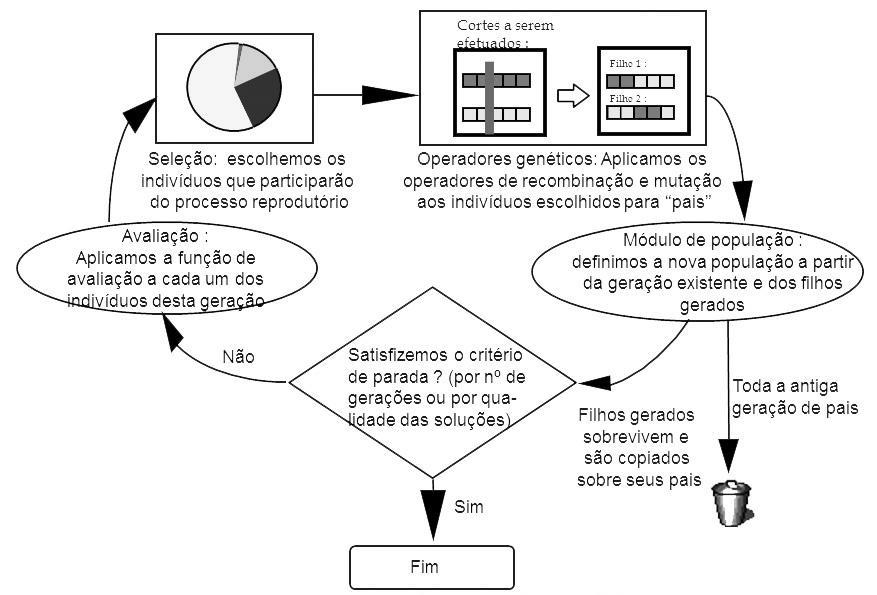
\includegraphics[scale=0.6]{imagens/revisao-bibliografica/esquemaAlgGenetico_pag64.png}
	\legend{Fonte: \citeonline[p. 64]{linden2012}.}
    	\end{center}
    \end{figure}
    
Incluindo uma figura de autoria própria.
\begin{figure} [htb]
\begin{center}
	 \caption{\label{fig:ambiente}Ambiente abordado}
	    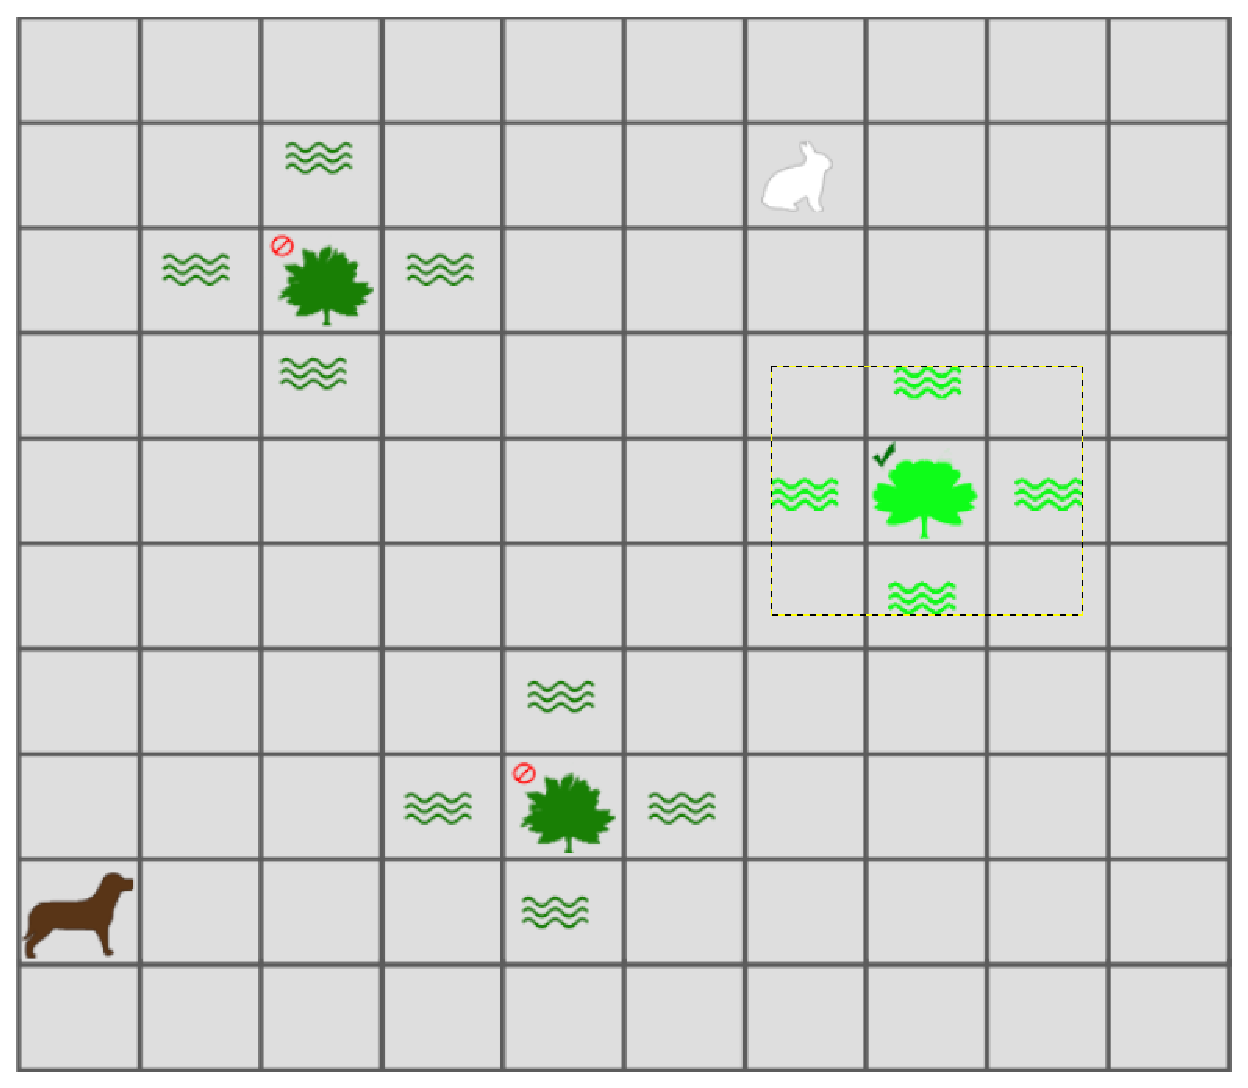
\includegraphics[scale=0.3]{imagens/revisao-bibliografica/ambiente.eps}
	\legend{Fonte: autoria própria.}
    \end{center}
\end{figure}

\subsection{tema 1 relacionado ao trabalho}



\subsection{tema 2 relacionado ao trabalho}


Exemplo 1 de citação, \cite{almeida2022}

Exemplo 2 de citação, \citeonline{almeida2022}\\ \\
% Deixar duas (2) linhas em branco antes do o título de uma seção
Lista com citações de  diferentes tipos de documentos, para gerar o exemplo de\\ \textbf{Referências} ao final do documento.\\ \\
Dissertação, \cite{almeida2022}\\
Trabalho publicado em Conferência, \cite{cbsoft2023}\\
Página web, \cite{ferreira2020}\\
Manual, \cite{latex2023}\\
Capitulo de livro, \cite{mendes2019}\\
Relatório técnico, \cite{oliveira2020}\\
Livro, \cite{linden2012}\\
Tese de doutorado, \cite{rodrigues2021}\\
Artigo científico, \cite{silva2023}\\
Livro de Conferência, \cite{souza2022}


% %%%%%%%%%%%%%%%%%%%%%%%%%%%%%%%%%%%%%%%%%%%%%%%%%%%%%%%%%%%%%%%%%%%%%%%%%%
\section{ATIVIDADES DESENVOLVIDAS} \label{ch:atividades-desenvolvidas}
% %%%%%%%%%%%%%%%%%%%%%%%%%%%%%%%%%%%%%%%%%%%%%%%%%%%%%%%%%%%%%%%%%%%%%%%%%%
Descreva em detalhes todas as atividades realizadas no estágio, explicando sua importância e os desafios enfrentados.

Crie subseções para dividir as diferentes atividades e etapas  envolvidas no estágio.

% -------------------------------------------------------------------------
\subsection{ Seção Atividade Parcial 1} \label{sec:definir-tituto-da-secao1}
% -------------------------------------------------------------------------

Discussão detalhada de um dos tópicos fundamentais para o entendimento do problema abordado. \\ Caso necessário, pode ser criado subseções

Para referenciar a tabela você pode usar o comando "autoref" ex: \autoref{tab:resultados1}, ou o "ref", ex: \ref{tab:resultados1}

\begin{table}[htb]
\centering
\caption{Exemplo de tabela conforme a ABNT}
\label{tab:resultados1}
\begin{tabular}{p{0.3\textwidth} p{0.3\textwidth} p{0.3\textwidth}} % Ajuste das larguras das colunas
    \hline
    \textbf{Coluna 1} & \textbf{Coluna 2} & \textbf{Coluna 3} \\
    \hline
    Informação 1 & Informação 2 & Informação 3 \\
    Informação 4 & Informação 5 & Informação 6 \\
    Informação 7 & Informação 8 & Informação 9 \\  
    \hline
\end{tabular}
\legend{Fonte: autoria própria.}
\end{table}

\begin{table}[htb]
\centering
\caption{Exemplo de tabela conforme a ABNT}
\label{tab:resultados2}
\begin{tabular}{>{\centering\arraybackslash}p{0.3\textwidth}  >{\centering\arraybackslash}p{0.3\textwidth}  >{\centering\arraybackslash}p{0.3\textwidth}} % Ajuste das larguras das colunas
    \hline
    \textbf{Coluna 1} & \textbf{Coluna 2} & \textbf{Coluna 3} \\
    \hline
    Informação 1 & Informação 2 & Informação 3 \\
    Informação 4 & Informação 5 & Informação 6 \\
    Informação 7 & Informação 8 & Informação 9 \\  
    \hline
\end{tabular}
\legend{Fonte: autoria própria.}
\end{table}


\begin{table}[ht]
    \centering
    \caption{Exemplo de tabela conforme a ABNT}
    \label{quad:exemplo}
    \begin{tabular}{p{3cm} p{4cm} p{3cm}}
        \hline%\toprule
        \textbf{Coluna 1} & \textbf{Coluna 2} & \textbf{Coluna 3} \\
        \hline%\midrule
        Informação 1 & Informação 2 & Informação 3 \\
        Informação 4 & Informação 5 & Informação 6 \\
        Informação 7 & Informação 8 & Informação 9 \\
        \hline%\bottomrule
    \end{tabular}
    \legend{Fonte: \citeonline{linden2012}.}
\end{table}



% -------------------------------------------------------------------------
\subsection{ Seção Atividade Parcial 2} \label{sec:definir-tituto-da-secao2}
% -------------------------------------------------------------------------

Discussão detalhada de um dos tópicos fundamentais para o entendimento do problema abordado. \\ Caso necessário, pode ser criado subseções


% %%%%%%%%%%%%%%%%%%%%%%%%%%%%%%%%%%%%%%%%%%%%%%%%%%%%%%%%%%%%%%%%%%%%%%%%%%
\section{Considerações Finais} \label{ch:consideracoes-finais}
% %%%%%%%%%%%%%%%%%%%%%%%%%%%%%%%%%%%%%%%%%%%%%%%%%%%%%%%%%%%%%%%%%%%%%%%%%%
Resuma as principais contribuições do trabalho, avalie o cumprimento dos objetivos definidos na seção \textbf{Objetivos} e sugira possíveis direções para trabalhos futuros.\\
Além disso, reflita sobre a experiência do estágio, destacando os principais aprendizados, os desafios superados e o impacto na sua formação. 


% ******************************************************************************
%				           ELEMENTOS PÓS-TEXTUAIS				               *
% ******************************************************************************
\postextual
% ----------------------------------------------------------

\bibliography{references}

% ----------------------------------------------------------
% Glossário
% ----------------------------------------------------------
%
% Consulte o manual da classe abntex2 para orientações sobre o glossário.
%
%\glossary

% ----------------------------------------------------------
% Apêndices
% ----------------------------------------------------------

% ---
% Inicia os apêndices
% ---
%\begin{apendicesenv}

% Imprime uma página indicando o início dos apêndices
%\partapendices

% ----------------------------------------------------------
%\chapter{Quisque libero justo}
% ----------------------------------------------------------

%\lipsum[50]

% ----------------------------------------------------------
%\chapter{Nullam elementum urna vel imperdiet sodales elit ipsum pharetra ligula
%ac pretium ante justo a nulla curabitur tristique arcu eu metus}
% ----------------------------------------------------------
%\lipsum[55-57]

%\end{apendicesenv}
% ---


% ----------------------------------------------------------
% Anexos
% ----------------------------------------------------------

% ---
% Inicia os anexos
% ---
% \begin{anexosenv}

% % Imprime uma página indicando o início dos anexos
% %\partanexos
% % ---
% \chapter{Titulo anexo 1}
% % ---
% \lipsum[30]

% % % ---
% % \chapter{Cras non urna sed feugiat cum sociis natoque penatibus et magnis dis
% % parturient montes nascetur ridiculus mus}
% % % ---

% % \lipsum[31]


% \end{anexosenv}

%---------------------------------------------------------------------
% INDICE REMISSIVO
%---------------------------------------------------------------------
%\phantompart
%\printindex
%---------------------------------------------------------------------




% ------------ fim do documento ------------
\end{document}